\section{Aufbau und Durchführung}
Der Aufbau des Versuchs ist schematisch in Abblidung \ref{aufbau} dargestellt. Die zu untersuchende Probe (Sample tube) wird zwischen zwei starke Permanentmagnete positioniert. Zwei Sweep Coils erzeugen ein zusätzliches magnetisches Wechselfeld, das dem permanenten Magnetfeld überlagert ist. Am Radiofrequenz-Transmitter wird mit einem Rad eine Radiofrequenz eingestellt, mit der dann Radiowellen auf die Probe emittiert werden. Die Frequenz wird durch einen Frequenzzähler angezeigt. Um die Probe ist eine Spule angebracht, die zusammen mit einem Schaltkreis im Radiofrequenz-Empfänger als Detektor für die Absorbtion der Radiowellen in der Probe fungiert. Durch die Ausrichtung der nuklearen Spins ändert sich die Permeabilität und dadurch auch die Induktivität der Spule, was gemessen werden kann. Dann wird das Signal verstärkt und genau wie das Signal der Sweep Coils an das Oszilloskop gegeben, wie man in Abblidung \ref{oszi} sehen kann.
\begin{figure}[htbp] 
     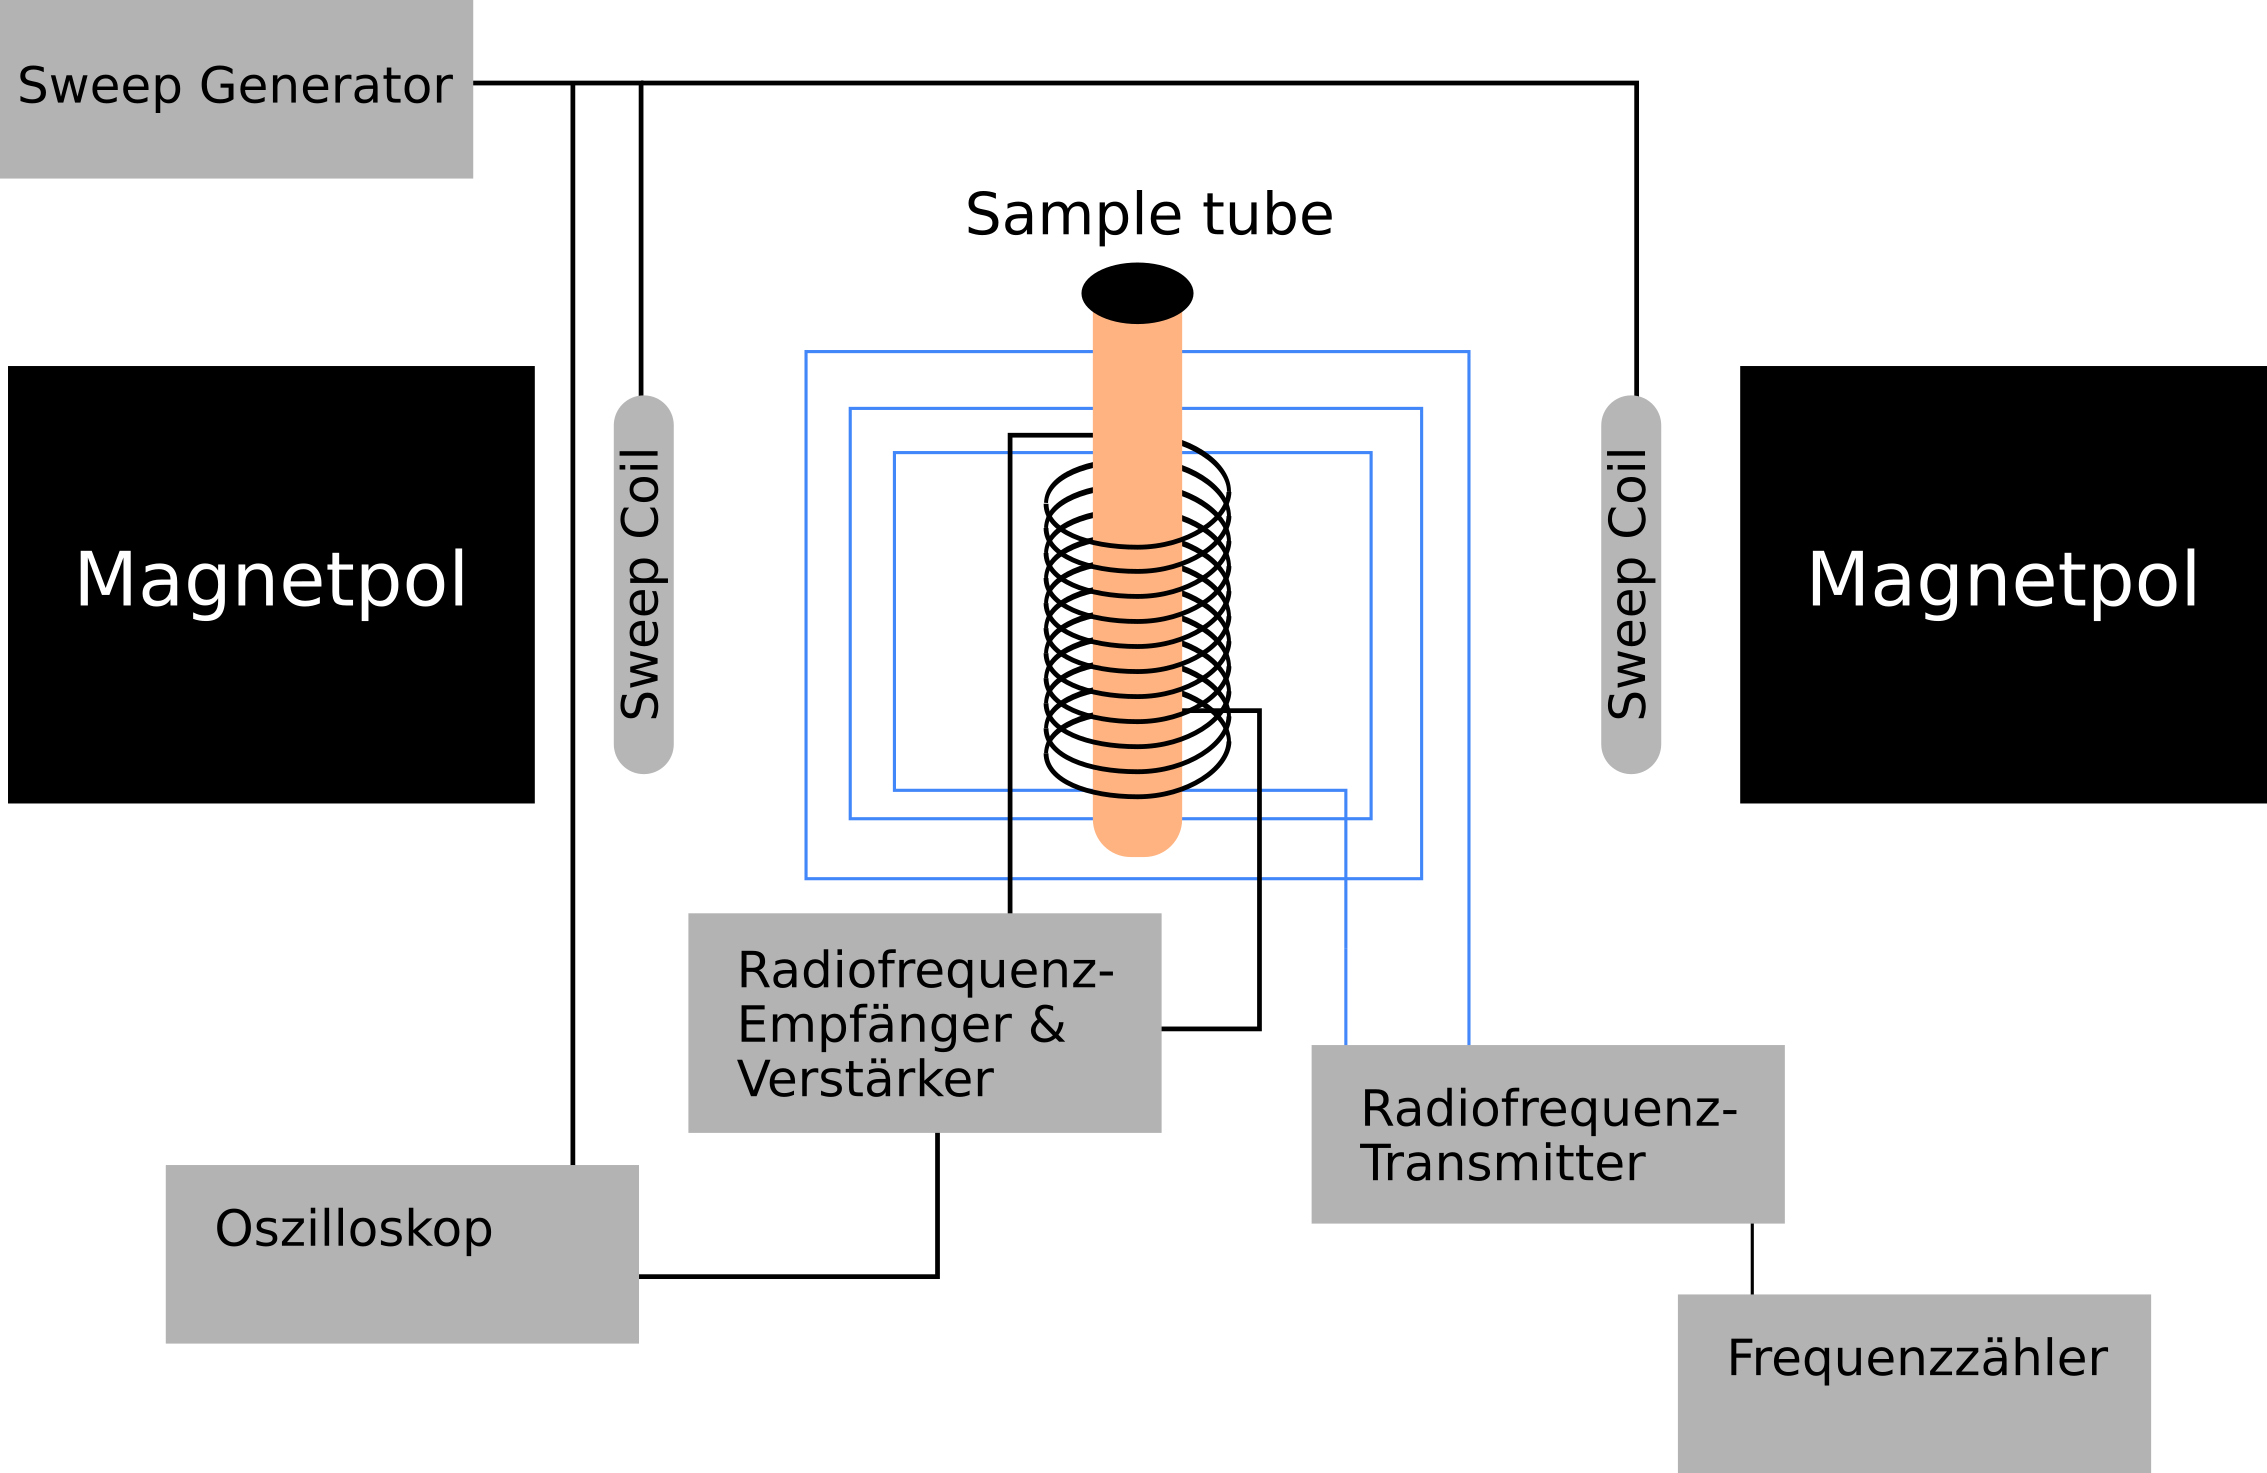
\includegraphics[width=0.99\textwidth]{Aufbau.png}
  \caption{Schematischer Aufbau der Versuchsinstrumente}
  \label{aufbau}
\end{figure}

\begin{figure}[htbp] 
     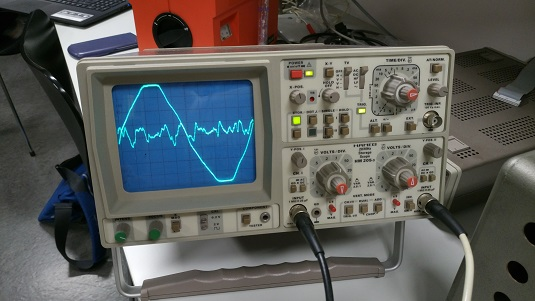
\includegraphics[scale=0.5]{Oszi.jpg}
  \caption{Oszilloskop mit Wechselmagnetfeld und Detektorsignal}
  \label{oszi}
\end{figure}

Durch das magnetische Wechselfeld erreicht man, dass die Aufspaltung der Energieniveaus erfolgt, aber auch dass die Besetzung der Energieniveaus nach einer gewissen Zeit nicht gleichverteilt ist. Dies würde dazu führen, dass keine Absorbtion der Radiowellen mehr erkennbar ist. Der Grund dafür ist, dass die Relaxationszeit aufgrund der geringen Energien sehr lang ist. Bei einem statischen Magnetfeld würde also die Absorbtion nach einer gewissen Zeit aufhören und die Relaxation in das thermodynamische Gleichgewicht, in der wieder Absorbtion stattfinden kann, würde zu lange dauern.

Die Durchführung des Versuchs beginnt damit, die Kalibrierung des Magnetfelds vorzunehmen. Von nun an darf die Halterung der Probe nicht mehr verändert werden, damit sich keine Änderungen des Magnetfelds ergeben, die nicht einberechnet werden können. Für jede Probe wird das gleiche magnetische Wechselfeld angelegt und dann auf dem Oszillskop nach den Absorbtionspeaks innerhalb des Rauschens gesucht, während die Frequenz an dem Rad verändert wird. Für minimales und maximales Magnetfeld werden die Peaks gesucht und die zugehörige Frequenz wird so bestimmt, dass die von den Flanken des Magnetfelds kommenden Peaks irgendwann ineinander laufen. Dort wird dann die Frequenz am Frequenzzähler abgelesen. Die hohe und die niedrige Frequenz werden abwechselnd gesucht, jeweils 10 mal, sodass durch sich immer wiederholendes Neueinstellen der Frequenz eine gute Statistik entsteht.
